% generated by scripts/pkl_to_latex.py
% source PKL : vscan_v1_L8_Ne8_U10_t1_mode-uniform_nmin2_solver-gcg_sz0_restarts8_iter200_kmax4_tol1em09_V0to15_N16-2f7c06936fa2.pkl
% scan type  : vscan
% state      : gs
% requires   : \usepackage{pgfplots} \pgfplotsset{compat=1.18}
% colours match the matplotlib PDF (tab10 cycle)
\definecolor{gmeC0}{HTML}{1F77B4}
\definecolor{gmeC1}{HTML}{FF7F0E}
\definecolor{gmeC2}{HTML}{2CA02C}
\definecolor{gmeC3}{HTML}{D62728}
\definecolor{gmeC4}{HTML}{9467BD}
\definecolor{gmeC5}{HTML}{8C564B}
\definecolor{gmeC6}{HTML}{E377C2}
\definecolor{gmeC7}{HTML}{17BECF}

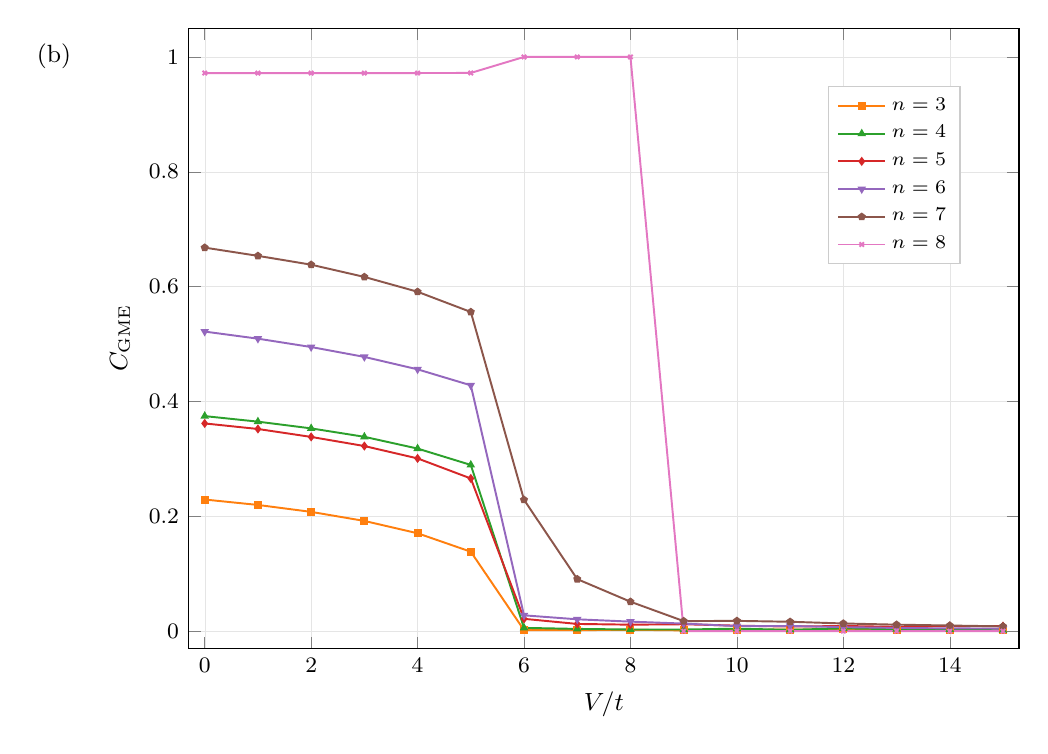
\begin{tikzpicture}
  \begin{axis}[
    width=\columnwidth,
    height=0.78\columnwidth,
    xlabel={$V/t$},
    ylabel={$C_{\mathrm{GME}}$},
    grid=both,
    grid style={line width=.1pt, draw=gray!20},
    tick label style={font=\footnotesize\rmfamily, /pgf/number format/fixed},
    label style={font=\small\rmfamily},
    scaled ticks=false,
    legend style={font=\scriptsize\rmfamily, draw=gray!40, at={(0.5,1.03)}, anchor=south, /tikz/every even column/.append style={column sep=6pt}},
    legend cell align={left},
    legend columns=1,
    ymin=-0.03,
    ymax=1.05,
    xmin=-0.3,
    xmax=15.3,
    legend style={at={(0.850,0.763)}, anchor=center, fill=white},
    after end axis/.append code={\node[anchor=east, font=\small\rmfamily] at (axis description cs:-0.13,0.954) {(b)};},
  ]
    \addplot[color=gmeC1, mark=square*, mark size=1.1pt, line width=0.7pt] coordinates {
        (0,0.229253) (1,0.219812) (2,0.207754) (3,0.191984)
        (4,0.170501) (5,0.138365) (6,0.001754) (7,0.001699)
        (8,0.002492) (9,0.001336) (10,0.002303) (11,0.002695)
        (12,0.003313) (13,0.001724) (14,0.002015) (15,0.001556)
    };
    \addlegendentry{$n=3$}
    \addplot[color=gmeC2, mark=triangle*, mark size=1.1pt, line width=0.7pt] coordinates {
        (0,0.374538) (1,0.36486) (2,0.353143) (3,0.338475)
        (4,0.317972) (5,0.2895) (6,0.005731) (7,0.003946)
        (8,0.002913) (9,0.002868) (10,0.004382) (11,0.002359)
        (12,0.004903) (13,0.003497) (14,0.00313) (15,0.001293)
    };
    \addlegendentry{$n=4$}
    \addplot[color=gmeC3, mark=diamond*, mark size=1.1pt, line width=0.7pt] coordinates {
        (0,0.361761) (1,0.352094) (2,0.338272) (3,0.32239)
        (4,0.300857) (5,0.265945) (6,0.021494) (7,0.012596)
        (8,0.01131) (9,0.012061) (10,0.009614) (11,0.007998)
        (12,0.009035) (13,0.007557) (14,0.008977) (15,0.008823)
    };
    \addlegendentry{$n=5$}
    \addplot[color=gmeC4, mark=triangle*, mark size=1.1pt, mark options={rotate=180}, line width=0.7pt] coordinates {
        (0,0.521727) (1,0.509364) (2,0.494826) (3,0.477628)
        (4,0.455968) (5,0.428151) (6,0.027587) (7,0.020662)
        (8,0.016613) (9,0.013227) (10,0.008797) (11,0.009076)
        (12,0.007004) (13,0.005626) (14,0.004816) (15,0.004539)
    };
    \addlegendentry{$n=6$}
    \addplot[color=gmeC5, mark=pentagon*, mark size=1.1pt, line width=0.7pt] coordinates {
        (0,0.667936) (1,0.6536) (2,0.638193) (3,0.616905)
        (4,0.591054) (5,0.555854) (6,0.228773) (7,0.090651)
        (8,0.051287) (9,0.017551) (10,0.017938) (11,0.016398)
        (12,0.013404) (13,0.011341) (14,0.009842) (15,0.008368)
    };
    \addlegendentry{$n=7$}
    \addplot[color=gmeC6, mark=x, mark size=1.1pt, line width=0.7pt] coordinates {
        (0,0.97189) (1,0.971892) (2,0.971898) (3,0.971911)
        (4,0.97195) (5,0.972117) (6,1) (7,1)
        (8,1) (9,0) (10,0) (11,0)
        (12,0) (13,0) (14,0) (15,0)
    };
    \addlegendentry{$n=8$}
  \end{axis}
\end{tikzpicture}
